\chapter{Supernova Neutrino Bursts and Low-energy Neutrinos}
\label{ch:physics-snblowe}

\section{Overview}
\label{sec:physics-snblowe-overview}

The DUNE experiment will be sensitive to neutrinos in the few
tens of MeV range, which create short electron tracks in liquid argon, potentially accompanied by a few
gamma rays. % and other secondary particle signatures.   
This regime is of
particular interest for detection of the burst of neutrinos from a galactic
core-collapse supernova (the primary focus of this chapter). 
The sensitivity of DUNE is primarily to \textit{electron flavor} supernova neutrinos, and this capability is unique among existing and proposed supernova neutrino detectors for the next decades.  
Neutrinos from other astrophysical sources are also potentially detectable.  
The low-energy event regime has several reconstruction, background and triggering challenges. 

The observation of neutrinos from the celebrated SN1987A core
collapse~\cite{Bionta:1987qt,Hirata:1987hu} in the Large Magellanic
Cloud outside the Milky Way %were detected. This observation 
provided qualitative validation of the basic physical picture of core-collapse and provided powerful constraints on numerous models of new physics. At the same time, the statistics were sparse 
and many questions remain.  A high-statistics observation of a
nearby supernova neutrino burst would be possible with the current
generation of detectors. Such an observation would shed light on 
the nature of the astrophysical event, as well as on the nature of
neutrinos themselves.  Sensitivity to the different flavor components
of the flux is highly desirable.

\subsection{The Stages of Core Collapse} %About Neutrinos from Collapsed Stellar Cores}

As a result of nuclear burning throughout a massive star's lifetime, the %central 
inner region of the star forms an ``onion'' structure, with an iron core at the center surrounded by concentric shells of lighter elements (silicon, oxygen, neon, magnesium, carbon, etc.). Eventually the core collapses, causing 
a core-collapse supernova\footnote{In this chapter ``Supernova'' always refers to a ``core-collapse supernova.''}.
 
As the star ages, its iron core, at temperatures of $T\sim 10^{10}$ K and densities of $\rho \sim 10^{10}$ g/cm$^{3}$, continuously loses energy through neutrino emission caused by pair annihilation and plasmon decay. Since iron does not burn, there is no mechanism to replenish this lost energy within the core, and the core continues to contract and heat up. Meanwhile, the shells around it burn, producing iron that gravitates to the core, adding mass to it.  When the core reaches the critical mass of about $1.4 M_{\odot}$ of Fe, a stable configuration is no longer possible. At this point, as electrons are absorbed by the protons and some iron is disintegrated by thermal photons, the pressure support is suddenly removed and the core collapses essentially in free fall, reaching speeds of about a quarter of the speed of light. 
\footnote{Other collapse mechanisms are possible: an ``electron-capture'' supernova does not reach the final burning phase before highly degenerate electrons break apart nuclei and trigger a collapse.}


The collapse of the core suddenly halts after $\sim 10^{-2}$ seconds, as the density reaches nuclear (and up to supra-nuclear)  values. The core then bounces and a shock wave forms. The extreme physical conditions of this core, in particular the densities of order $10^{12}-10^{14}$ g/cm$^{3}$, create a medium that is opaque even to neutrinos; %, but cooler; 
the temperature of this core is %not more than 
$\lesssim$ 30 MeV, which is relatively \emph{cold}. At this stage, the gravitational energy of the collapse is stored mostly in the degenerate Fermi sea of electrons ($E_{F}\sim 200$ MeV) and electron neutrinos, which are in equilibrium with each other, and the core's lepton number is trapped.

%At the next stage, \fixme{something must happen to make the medium transparent to nu's; what?} 
A point is reached where the trapped energy and lepton number both escape 
%\fixme{This is weird, how does a number escape? Is it that the lepton number is no longer fixed at a value or something?}
from the core, carried by the least interacting particles, i.e., neutrinos, according to the Standard Model.  A tremendous amount of energy, some $10^{53}$ ergs, is released in a time span of a few seconds by $10^{58}$ neutrinos and antineutrinos of all flavors, with energies of $\sim 10$~MeV. 
A small fraction of this energy is absorbed by beta reactions that form a shock wave. This shock wave blasts away the rest of the star creating a spectacular explosion, which, curiously enough, is only a tiny perturbation from the energetics point of view. 
\fixme{This isn't  clear enough. Here's what I think it says: 1. core reaches critical mass. 2. core collapses. 3. density reaches critical point and core bounces back; shock wave forms. 4. gravitational energy of core now stored in fermi sea and neutrinos; core is now opaque to neutrinos? (seems like this would happen before bounce back starts). 5. something happens so that neutrinos can escape. 6. neutrinos escape with most of energy. 7. a shock wave forms from remaining energy and blasts away rest of star. 8. we're left with neutron star or black hole.  Please confirm or correct. Maury says it's correct, but too late to change text. 12/15/15}

Over 99\% of all gravitational binding energy of the $1.4 M_{\odot}$ collapsed core -- some 10\% of its rest mass -- has now been emitted as neutrinos. The resulting central object then settles to a neutron star or a black hole. 


\subsection{Observable Signals from the Explosion} %{Stages of the Explosion}

The flavor content and spectra of the neutrinos emitted from the neutrinosphere (the surface of neutrino trapping) change
throughout the phases of the core collapse, and the neutrino signal provides information on the supernova's evolution.  

The signal starts with a short, sharp
\emph{neutronization} (or \emph{break-out}) burst primarily composed of
$\nu_e$. %These neutrinos are messengers of the shock front breaking through the neutrinosphere (the surface of neutrino trapping): when this happens, iron is disintegrated, the neutrino scattering cross section drops and the lepton number trapped just below the original neutrinosphere is suddenly released. (This essentially repeats info in prev section}
This quick and intense burst is followed by an
\emph{accretion} phase lasting some hundreds of milliseconds, depending on the progenitor star mass, as matter falls onto the collapsed core and the shock is stalled at the distance of perhaps $\sim 200$ km. The gravitational binding energy of the accreting material powers the neutrino luminosity during this stage. The %later
\emph{cooling} phase that follows, %over 
lasting $\sim$10~seconds, represents the main part of
the signal, over which the proto-neutron star sheds its trapped energy.  

Some fairly generic features of the neutrinos emitted in each stage are illustrated in Figure~\ref{fig:spectrum}, based on a 1-dimensional model of~\cite{Fischer:2009af} and reproduced from~\cite{Wurm:2011zn}.
\begin{cdrfigure}[Expected core-collapse neutrino signal]{spectrum}{Expected
  core-collapse neutrino signal from the ``Basel''
  model~\cite{Fischer:2009af}, for a
  10.8 $M_{\odot}$ progenitor.  The left plots show the very early
  signal, including neutronization burst; the middle plots show
  the accretion phase, and the right plots show the cooling
  phase. Across the top, luminosities as a function of time are shown. 
  Across the bottom, the plots show average energy as a function of time for the
  $\nu_e$, $\overline{\nu}_e$ and $\nu_{\mu,\tau}$ flavor components of the
  flux (fluxes for $\nu_\mu$, $\overline{\nu}_\mu$, $\nu_\tau$,
  and $\overline{\nu}_\tau$ should be identical).  Figure courtesy of~\cite{Wurm:2011zn}.}
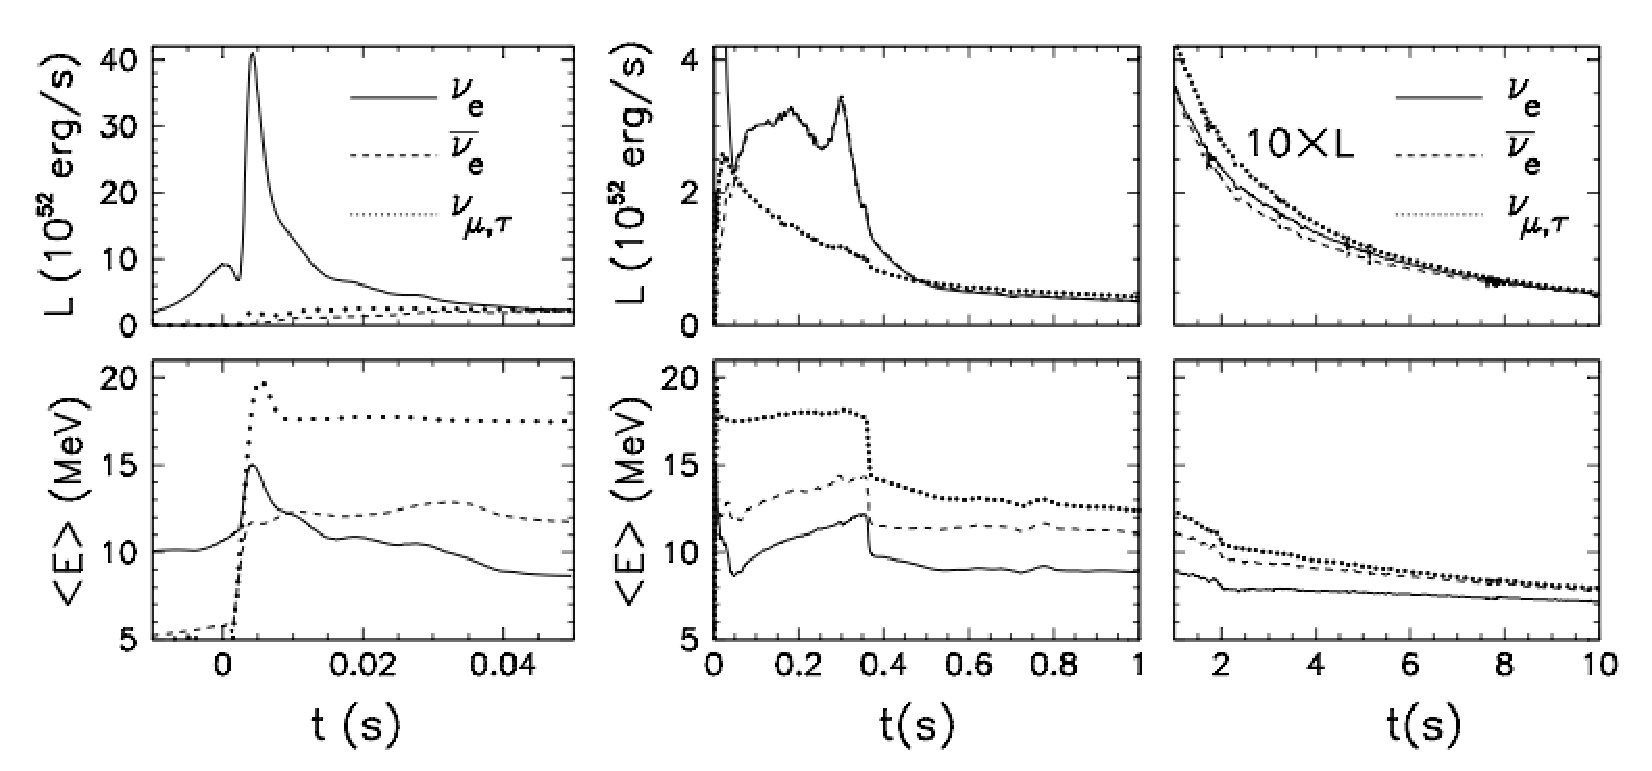
\includegraphics[width=0.9\textwidth]{basel_flux.pdf}
\end{cdrfigure}

The physics of neutrino decoupling and spectrum formation is far from trivial, owing to the energy dependence of the cross sections and the roles played by both charged- and neutral-current reactions.
Detailed transport calculations using methods such as Monte Carlo or Boltzmann solvers have been employed. It has been observed that spectra coming out of such simulations can typically be parameterized at a given moment in time by the following ansatz (e.g.,~\cite{Minakata:2008nc,Tamborra:2012ac}):
\begin{equation}
        \label{eq:pinched}
        \phi(E_{\nu}) = \mathcal{N} 
        \left(\frac{E_{\nu}}{\langle E_{\nu} \rangle}\right)^{\alpha} \exp\left[-\left(\alpha + 1\right)\frac{E_{\nu}}{\langle E_{\nu} \rangle}\right] \ ,
\end{equation}
where $E_{\nu}$ is the neutrino energy, $\langle E_\nu \rangle$ is the
mean neutrino energy, $\alpha$ is a ``pinching parameter,'' and
$\mathcal{N}$ is a normalization constant.
%
Large $\alpha$ corresponds to a more \emph{pinched} spectrum (suppressed
high-energy tail). This parameterization is referred to as a
\emph{pinched-thermal} form. The different $\nu_e$, $\overline{\nu}_e$ and
$\nu_x, \, x = \mu, \tau$ flavors are expected to have different
average energy and $\alpha$ parameters and to evolve differently in
time. 

The initial spectra get further processed (permuted) by flavor oscillations; understanding these oscillations is very important for extracting physics from the detected signal.

\subsection{Detection Channels and Interaction Rates in Liquid Argon}

Liquid argon has a particular sensitivity to the $\nu_e$ component of a supernova neutrino burst, via charged-current (CC)
absorption of $\nu_e$ on $^{40}$Ar,
\begin{equation}
\nu_e + ^{40}{\rm Ar} \rightarrow e^- + ^{40}{\rm K^*},
\label{eq:nueabs}
\end{equation}
for which the observables are the $e^-$ plus de-excitation products from the excited $K^*$ final state, as well as a $\bar{\nu}_e$ interaction and elastic scattering on electrons.
Cross sections for the most
relevant interactions are shown in Figure~\ref{fig:xscns}.

\begin{cdrfigure}[Cross sections for supernova-relevant interactions in argon]{xscns}{Cross sections for supernova-relevant interactions in argon~\cite{GilBotella:2003sz,snowglobes}.}
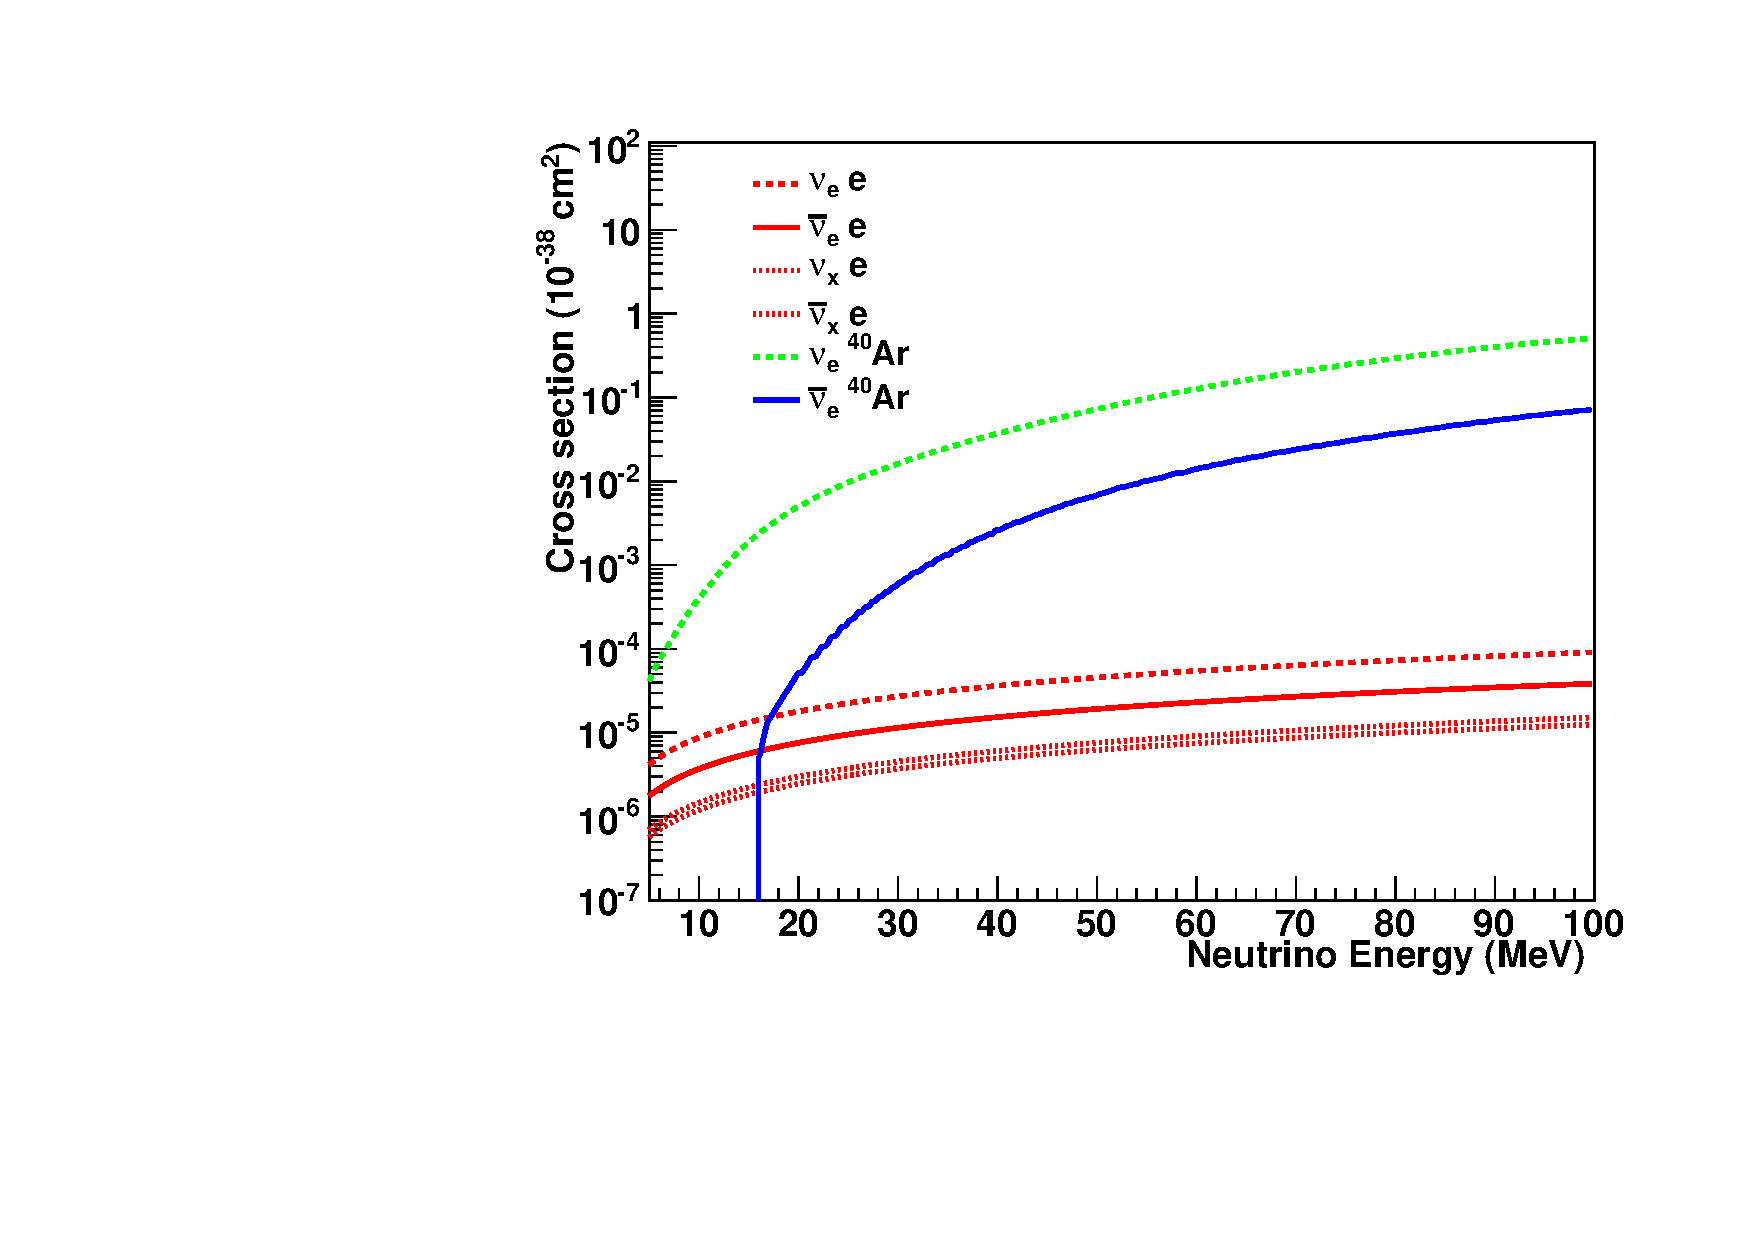
\includegraphics[width=0.6\textwidth]{argon_xscn.pdf}
\end{cdrfigure}

% From Flavio Another process of interest for supernova detection in LAr detectors, not yet fully studied, is neutral-current scattering on Ar nuclei by any type of neutrino: $\nu_x + {\rm Ar} \rightarrow \nu_x + {\rm Ar}^*$,  for which the signature is given by the cascade of de-excitation $\gamma$s from the final-state Ar nucleus. A dominant 9.8-MeV Ar$^*$ decay line has been recently identified as a spin-flip M1 transition~\cite{Hayes}.   At this energy the probability of $e^+e^-$ pair production is relatively high, offering a potentially interesting neutral-current tag.

Neutral-current (NC) scattering on Ar nuclei by any type of neutrino, $\nu_x + {\rm Ar} \rightarrow \nu_x + {\rm Ar}^*$, is another process of interest for supernova detection in LAr detectors that is not yet fully studied. The signature is given by the cascade of de-excitation $\gamma$s from the final-state Ar nucleus. A dominant 9.8-MeV Ar$^*$ decay line has been recently identified as a spin-flip M1 transition~\cite{Hayes}.   At this energy the probability of $e^+e^-$ pair production is relatively high, offering a potentially interesting neutral-current tag.

The predicted event rate (NC or CC) from a supernova burst may be calculated by
folding expected neutrino differential energy spectra in with cross
sections for the relevant channels and with detector response; this is done using SNOwGLoBES~\cite{snowglobes}, which uses Icarus detector resolution~\cite{Amoruso:2003sw} and assumes a detection threshold of 5~MeV.

Table~\ref{tab:argon_events} shows rates calculated  for the dominant interactions in argon for
the ``Livermore'' model~\cite{Totani:1997vj} (no longer preferred, but included for comparison with literature), and the ``GKVM''
model~\cite{Gava:2009pj}; for the former, no oscillations are assumed; the latter assumes collective oscillation effects (see Section~\ref{sec:physics-snblowe-neutrino-physics}). There is a rather wide variation --- up to an order of magnitude --- in event rate for different models, due to different numerical treatment (e.g., neutrino transport, dimensionality), physics input (nuclear equation of state, nuclear correlation and impact on neutrino opacities, neutrino-nucleus interactions) and oscillation effects. In addition, there is intrinsic variation in the nature of the progenitor and collapse mechanism.  
%\fixme{ Is it that the collapse mechanism for a particular type of progenitor can vary?  Maybe: `intrinsic variation in the collapse mechanism for a given type of progenitor'?  Maury says: leave as is}
 Furthermore, neutrino emission from the supernova may exhibit an emitted lepton-flavor asymmetry~\cite{Tamborra:2014aua}, which would lead to observed rates being direction-dependent.
\begin{cdrtable}[Event rates for different models in \SI{40}{\kt} of LAr for
    a core-collapse at 10~kpc]{lcc}{argon_events}{Event rates for different
    supernova models in \SI{40}{\kt} of liquid argon for a core collapse at 10~kpc, for $\nu_e$ and $\bar{\nu}_e$ charged-current channels and elastic scattering (ES) on electrons.
    Event rates will simply scale by active detector mass and inverse square of supernova distance. The ``Livermore'' model assumes no oscillations; ``GKVM'' assumes collective oscillation effects.  Oscillations (both standard and ``collective'') will potentially have a large, model-dependent effect.}
Channel & Events & Events \\
\rowtitlestyle
& ``Livermore'' model & ``GKVM'' model  \\ 
\toprowrule

$\nu_e + ^{40}{\rm Ar} \rightarrow e^- + ^{40}{\rm K^*}$ & 2720  & 3350 \\ \colhline

$\overline{\nu}_e + ^{40}{\rm Ar} \rightarrow e^+ + ^{40}{\rm Cl^*}$ & 230 & 160\\ \colhline

$\nu_x + e^- \rightarrow \nu_x + e^-$                           & 350 &  260\\ \colhline

Total &  3300 & 3770 \\ 
\end{cdrtable}



Figure~\ref{fig:garching} shows another example of an expected burst
signal, for which a calculation with detailed time-dependence of the
spectra is available~\cite{Huedepohl:2009wh} out to 9~seconds
post-bounce.  This model has relatively low luminosity but includes the standard robust
neutronization burst.   Note that the relative fraction of
neutronization-burst events is quite high.
Figure~\ref{fig:eventrates} shows the event channel breakdown for the same model.  Clearly, the $\nu_e$
flavor dominates.  Although other types of detectors, i.e., water and scintillator, have the capability to record $\nu_e$ events~\cite{Laha:2013hva,Laha:2014yua}, liquid argon offers the only prospect for observation of a large, clean supernova $\nu_e$ sample~\cite{Scholberg:2012id}.


\begin{cdrfigure}[Garching flux signal with neutronization burst]{garching}{Expected
  time-dependent signal for a specific flux model for an
  electron-capture supernova~\cite{Huedepohl:2009wh} at 10~kpc.  No oscillations are assumed. The
  top plot shows the luminosity as a function of time, the second plot
  shows average neutrino energy, and the third plot shows the $\alpha$
  (pinching) parameter.  The fourth (bottom) plot shows the total number of
  events (mostly $\nu_e$) expected in 40 kt of liquid argon, calculated using
  SNOwGLoBES.  Note the logarithmic binning in time; the plot shows
  the number of events expected in the given bin and the error bars
  are statistical. The vertical dashed line at 0.02 seconds indicates
  the time of core bounce, and the vertical lines indicate different
  eras in the supernova evolution.  The leftmost time interval
  indicates the infall period.  The next interval, from core bounce to
  50~ms, is the neutronization burst era, in which the flux is
  composed primarily of $\nu_e$.  The next period, from 50 to 200~ms,
  is the accretion period. The final era, from 0.2 to 9~seconds, is
  the proto-neutron-star cooling period.}
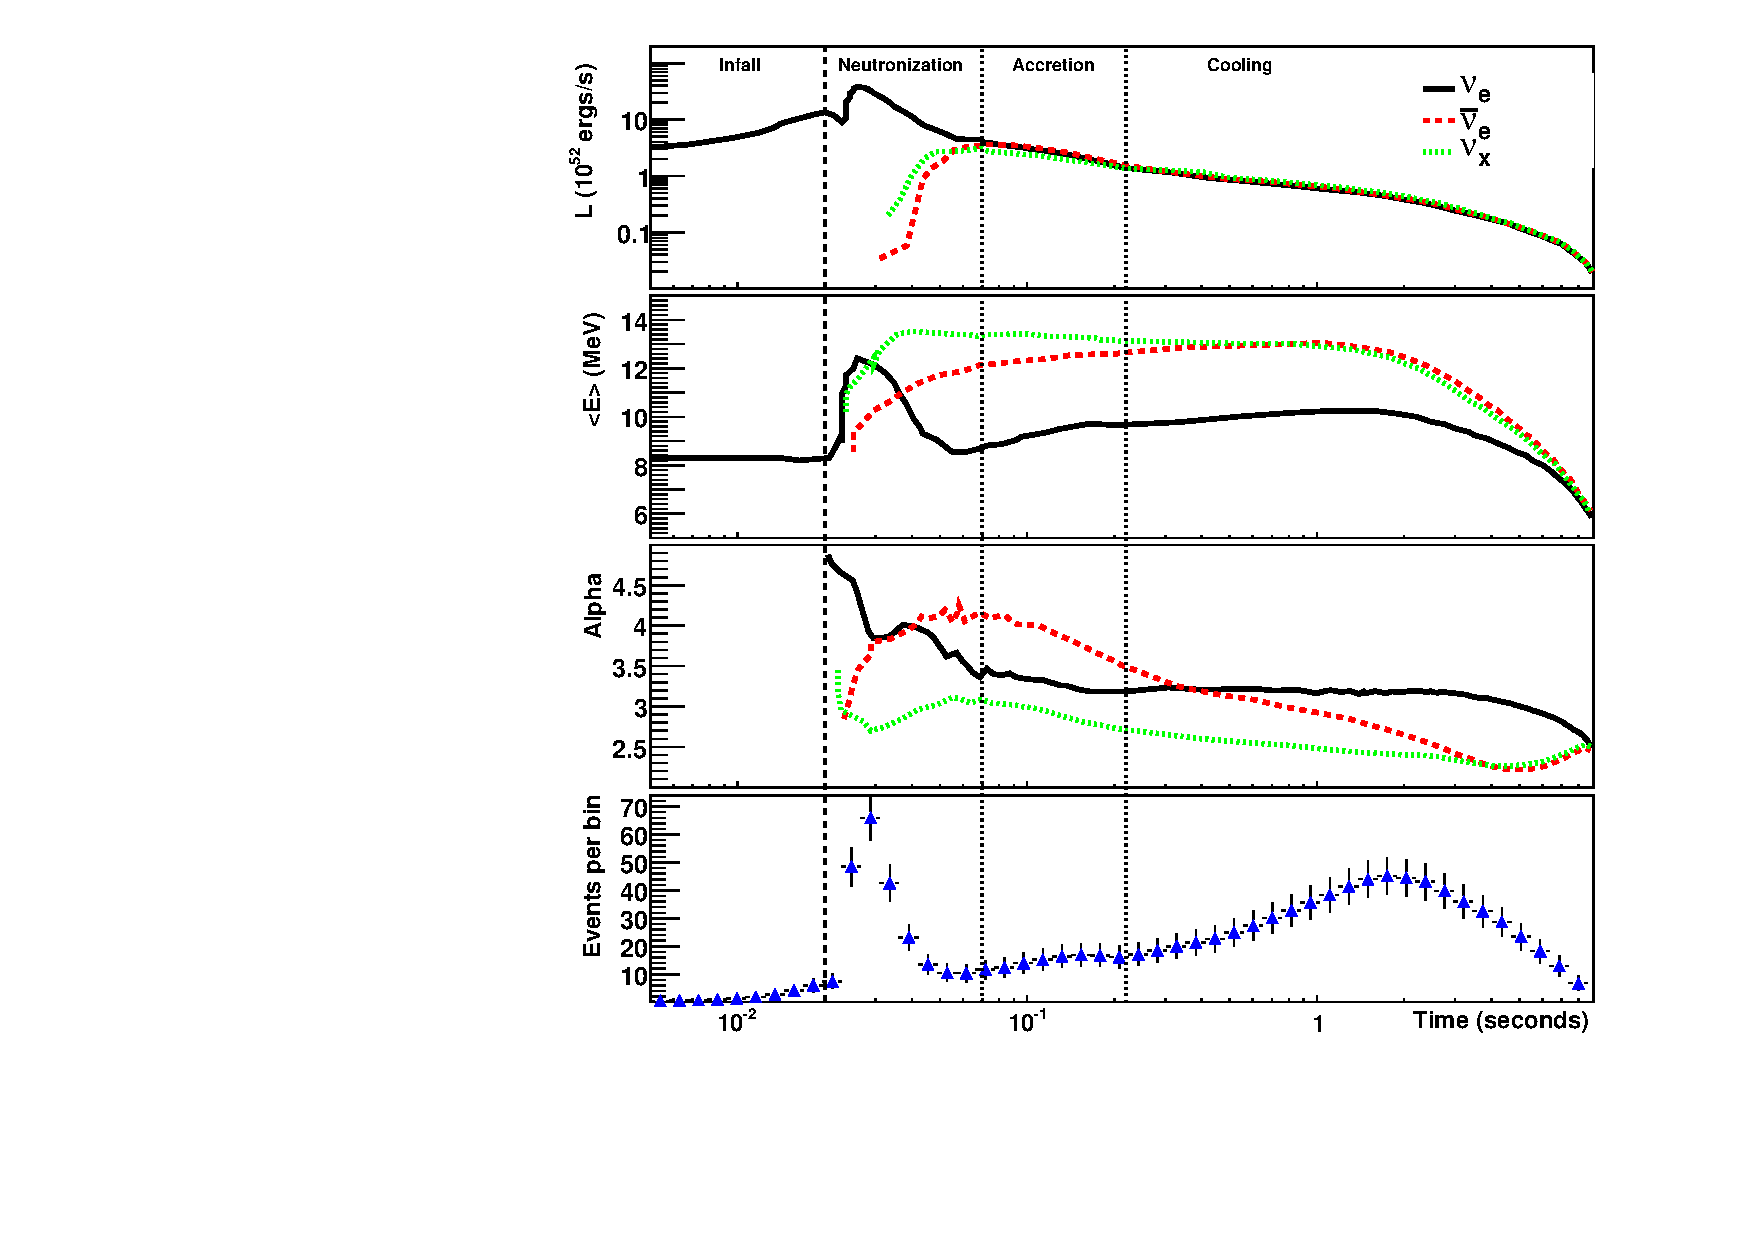
\includegraphics[width=0.9\textwidth]{garching.pdf}
\end{cdrfigure}


\begin{cdrfigure}[Supernova $\nu$ event rates in \SI{40}{kt} of LAr for Garching flux]{eventrates}{Left: Expected
  time-dependent signal in 40 kt of liquid argon for the electron-capture supernova~\cite{Huedepohl:2009wh} at 10~kpc, calculated using SNoWGLoBES~\cite{snowglobes}, showing breakdown of event channels.  Right: expected measured event spectrum for the same model, integrated over time.}
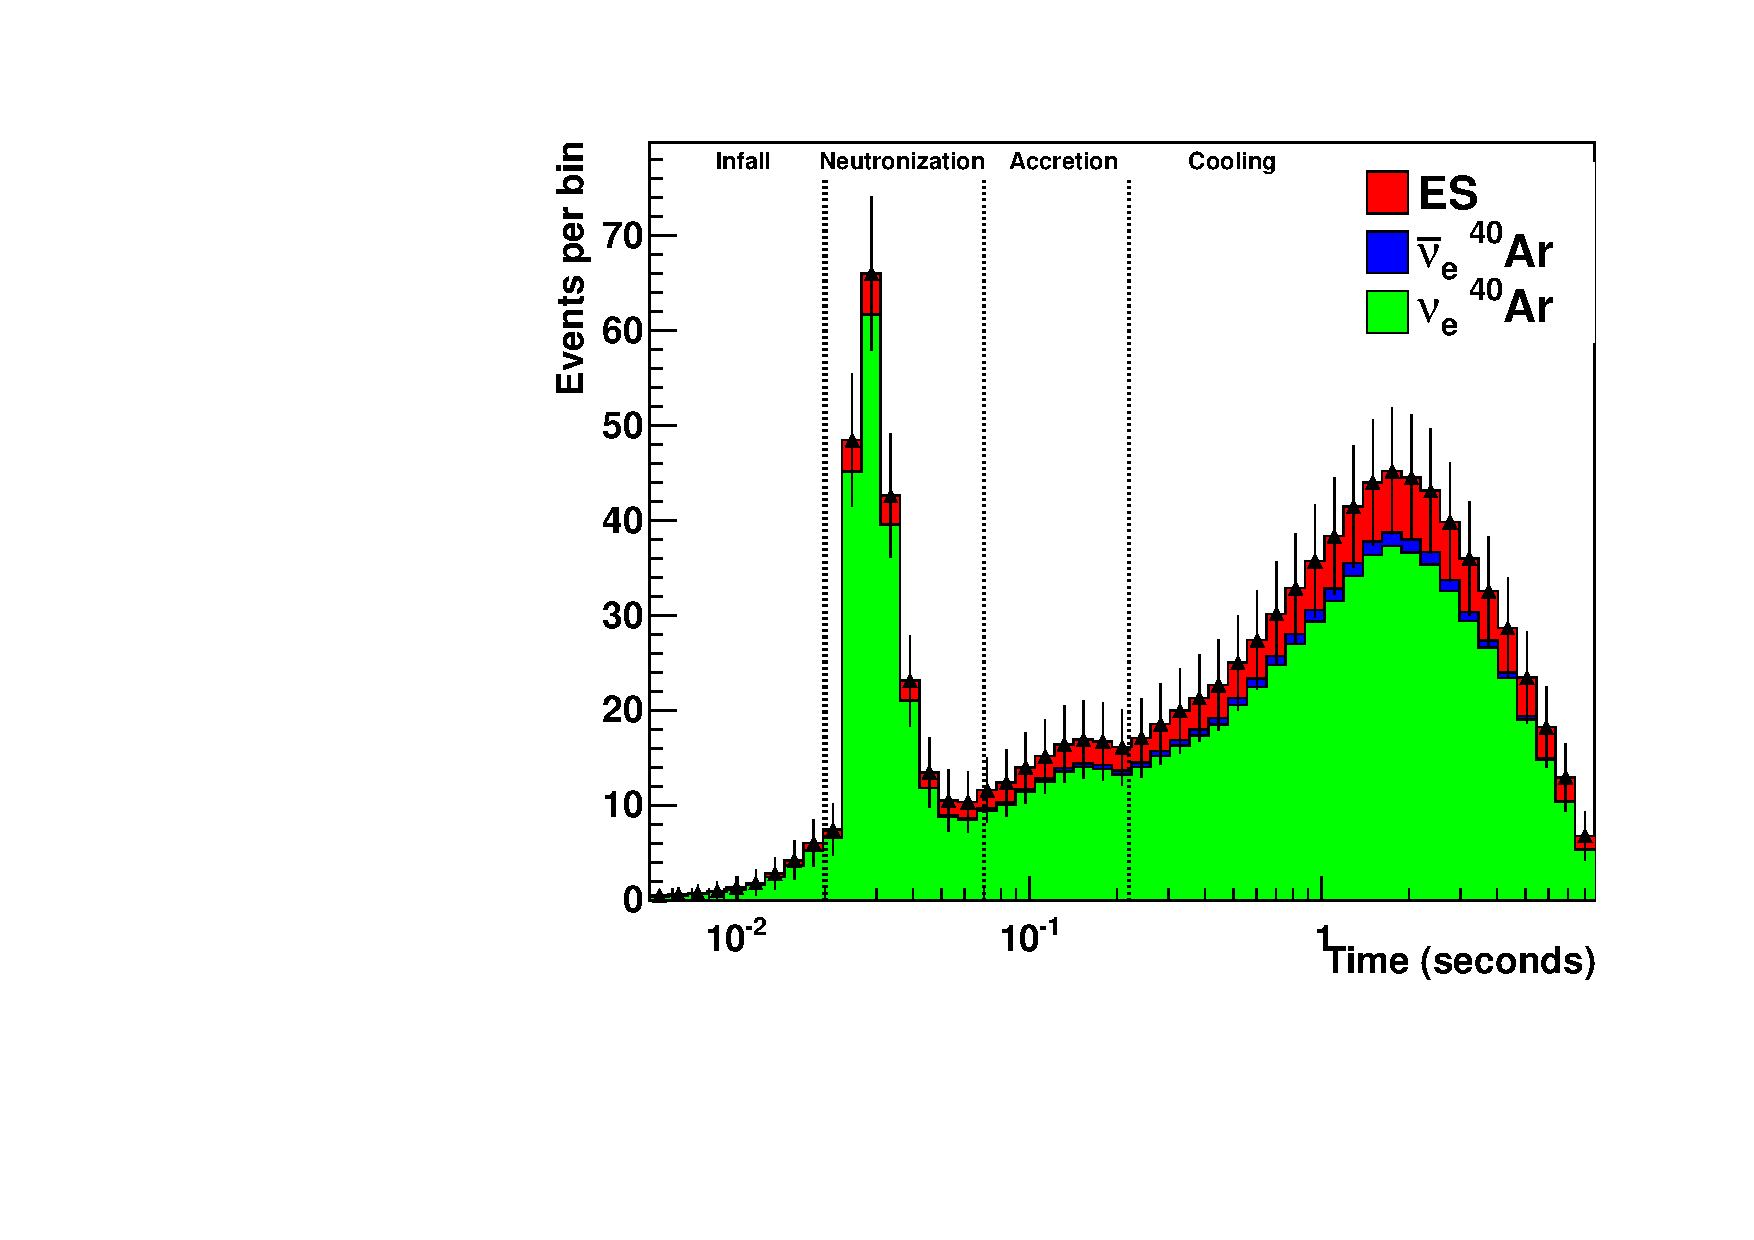
\includegraphics[width=2.5in]{garching_time_plot.pdf}
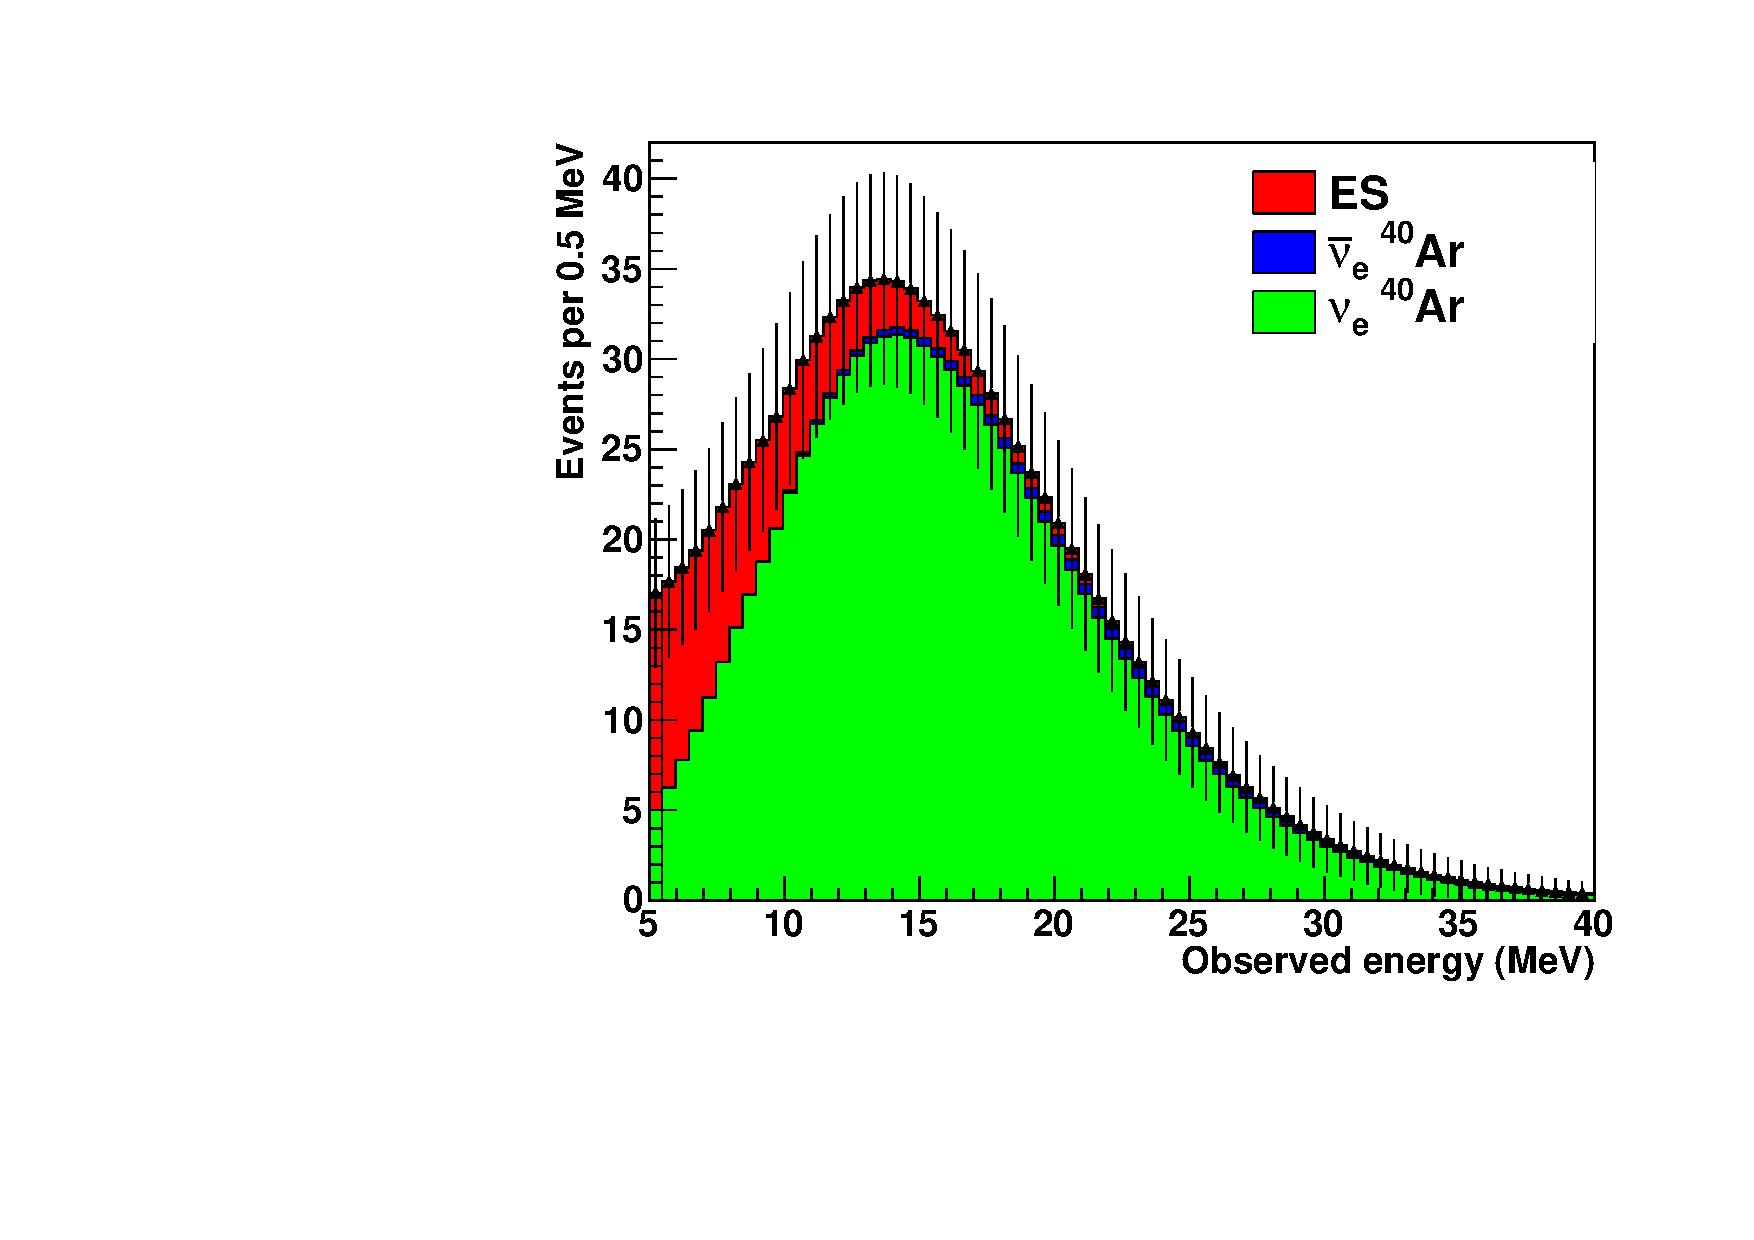
\includegraphics[width=2.5in]{garching_energy_plot.pdf}
\end{cdrfigure}

The number of signal events scales with mass and inverse square of distance as shown in Figure~\ref{fig:ratesvsdist}.  For a collapse in the Andromeda galaxy, a 40-kt detector would observe a few events.

\begin{cdrfigure}[Supernova neutrino rates vs. distance]{ratesvsdist}{Estimated numbers of supernova neutrino interactions in DUNE as a function of distance to the supernova, for different detector masses ($\nu_e$ events dominate). The red band 
represents expected events for a 40-kt detector and the green band represents expected events for a 10-kt detector. The borders of these bands (dashed lines) limit a fairly wide range of possibilities for ``Garching-parameterized'' supernova flux spectra (Equation~\ref{eq:pinched}) with luminosity $0.5\times 10^{52}$ ergs over ten seconds. The optimistic upper line of a pair gives the number of events for average $\nu_e$ energy of $\langle E_{\nu_e}\rangle =12$~MeV, and ``pinching'' parameter $\alpha=2$; the pessimistic lower line of a pair gives the number of events for $\langle E_{\nu_e}\rangle=8$~MeV and $\alpha=6$. (Note that the luminosity, average energy and pinching parameters will vary over the time frame of the burst, and these estimates assume a constant spectrum in time. Oscillations will also affect the spectra and event rates.) The solid lines represent the integrated number of events for the specific time-dependent neutrino flux model in~\cite{Huedepohl:2009wh} (see Figs.~\ref{fig:garching} and \ref{fig:eventrates}; this model has relatively cool spectra and low event rates). Core collapses are expected to occur a few times per century, at a most-likely distance of around 10 to 15 kpc.}
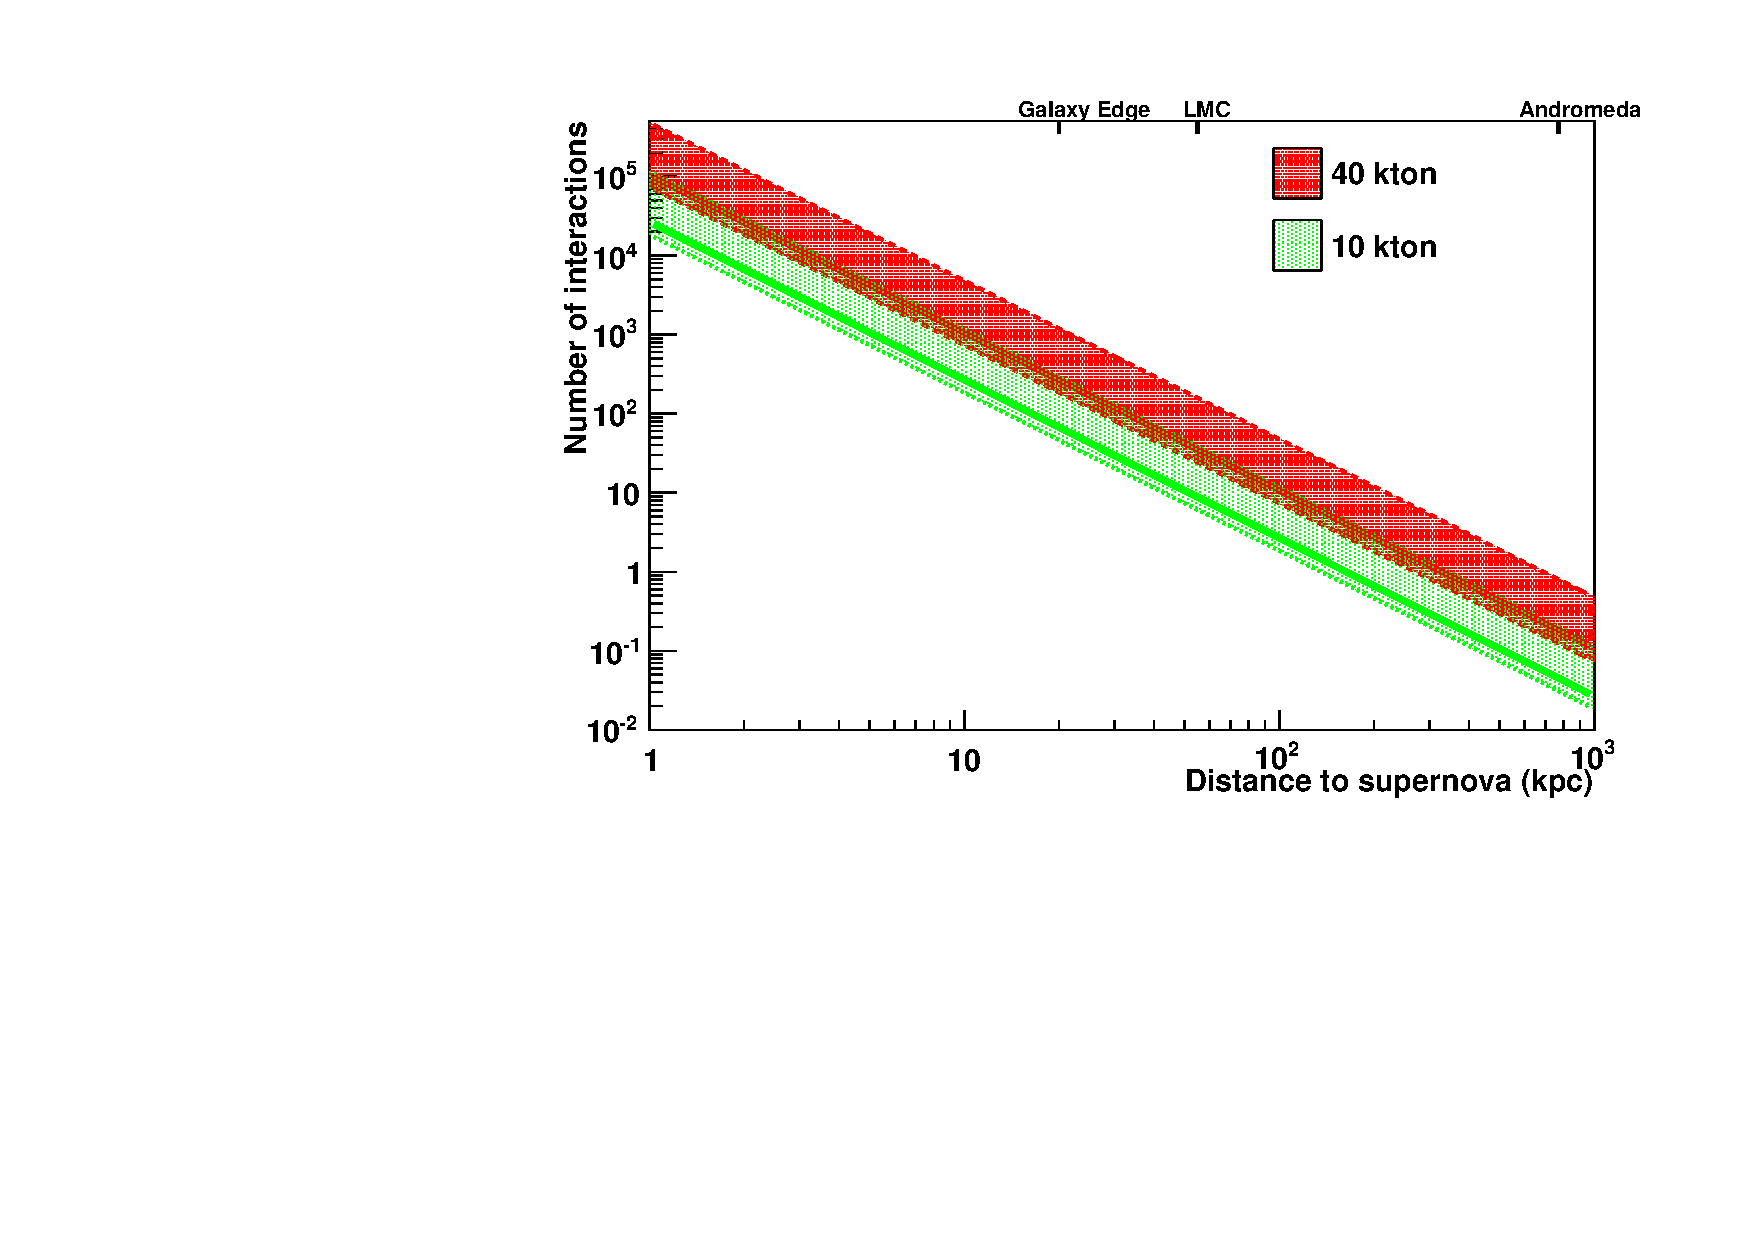
\includegraphics[width=5in]{argon_sn.pdf}
\end{cdrfigure}



\section{Neutrino Physics and Other Particle Physics}
\label{sec:physics-snblowe-neutrino-physics}

The key property of neutrinos that leads to a dominant role in supernova dynamics is the feebleness of their interactions. It then follows that should there be unknown, even weaker interactions or properties of neutrinos, or 
new, light ($< 100$ MeV) weakly interacting particles, they could alter the energy transport process and the resulting evolution of the nascent proto-neutron star. 
A core-collapse supernova can be thought of as %an extremely (it's either hermetic or it's not)
a hermetic system that can be used to search for numerous types of new physics (e.g.,~\cite{Schramm:1990pf,Raffelt:1999tx}). The list includes various Goldstone bosons (e.g., Majorons), neutrino magnetic moments, new gauge bosons (\emph{dark photons}), \emph{unparticles}, and extra-dimensional gauge bosons. %\fixme{Does this list jive with the section contents? Maury says it's ok} 
The existing data from SN1987A already provide significant constraints on these scenarios, by confirming the basic energy balance of the explosion. At the same time, more precision is highly desirable and should be provided by the next galactic supernova. 

\begin{cdrfigure}[Simulated cooling curves from the Garching light progenitor model]{coolingcurves}{ Average $\nu_{e}$ energy from a simulated fit to the oscillated fluxes predicted by the Garching 1D model with a light (10.8 $M_{\odot}$) progenitor. DUNE's oscillation calculations included full multi-angle treatment of collective evolution, for two
different mass hierarchy assumptions. The predicted events were then smeared with SNOwGLoBES and fit with a pinched-thermal spectrum as a function of time (assuming a supernova at 10 kpc and a 34 kt LAr detector). The bands represent $1\sigma$ error bars from the fit (assuming only statistical uncertainties). The solid black line is the true
$\langle E_{\nu} \rangle$ for the unoscillated spectrum. Clearly, the rate of energy escape from the proto-neutron star can be gleaned by tracking $\nu_{e}$ spectra as a function of time.}
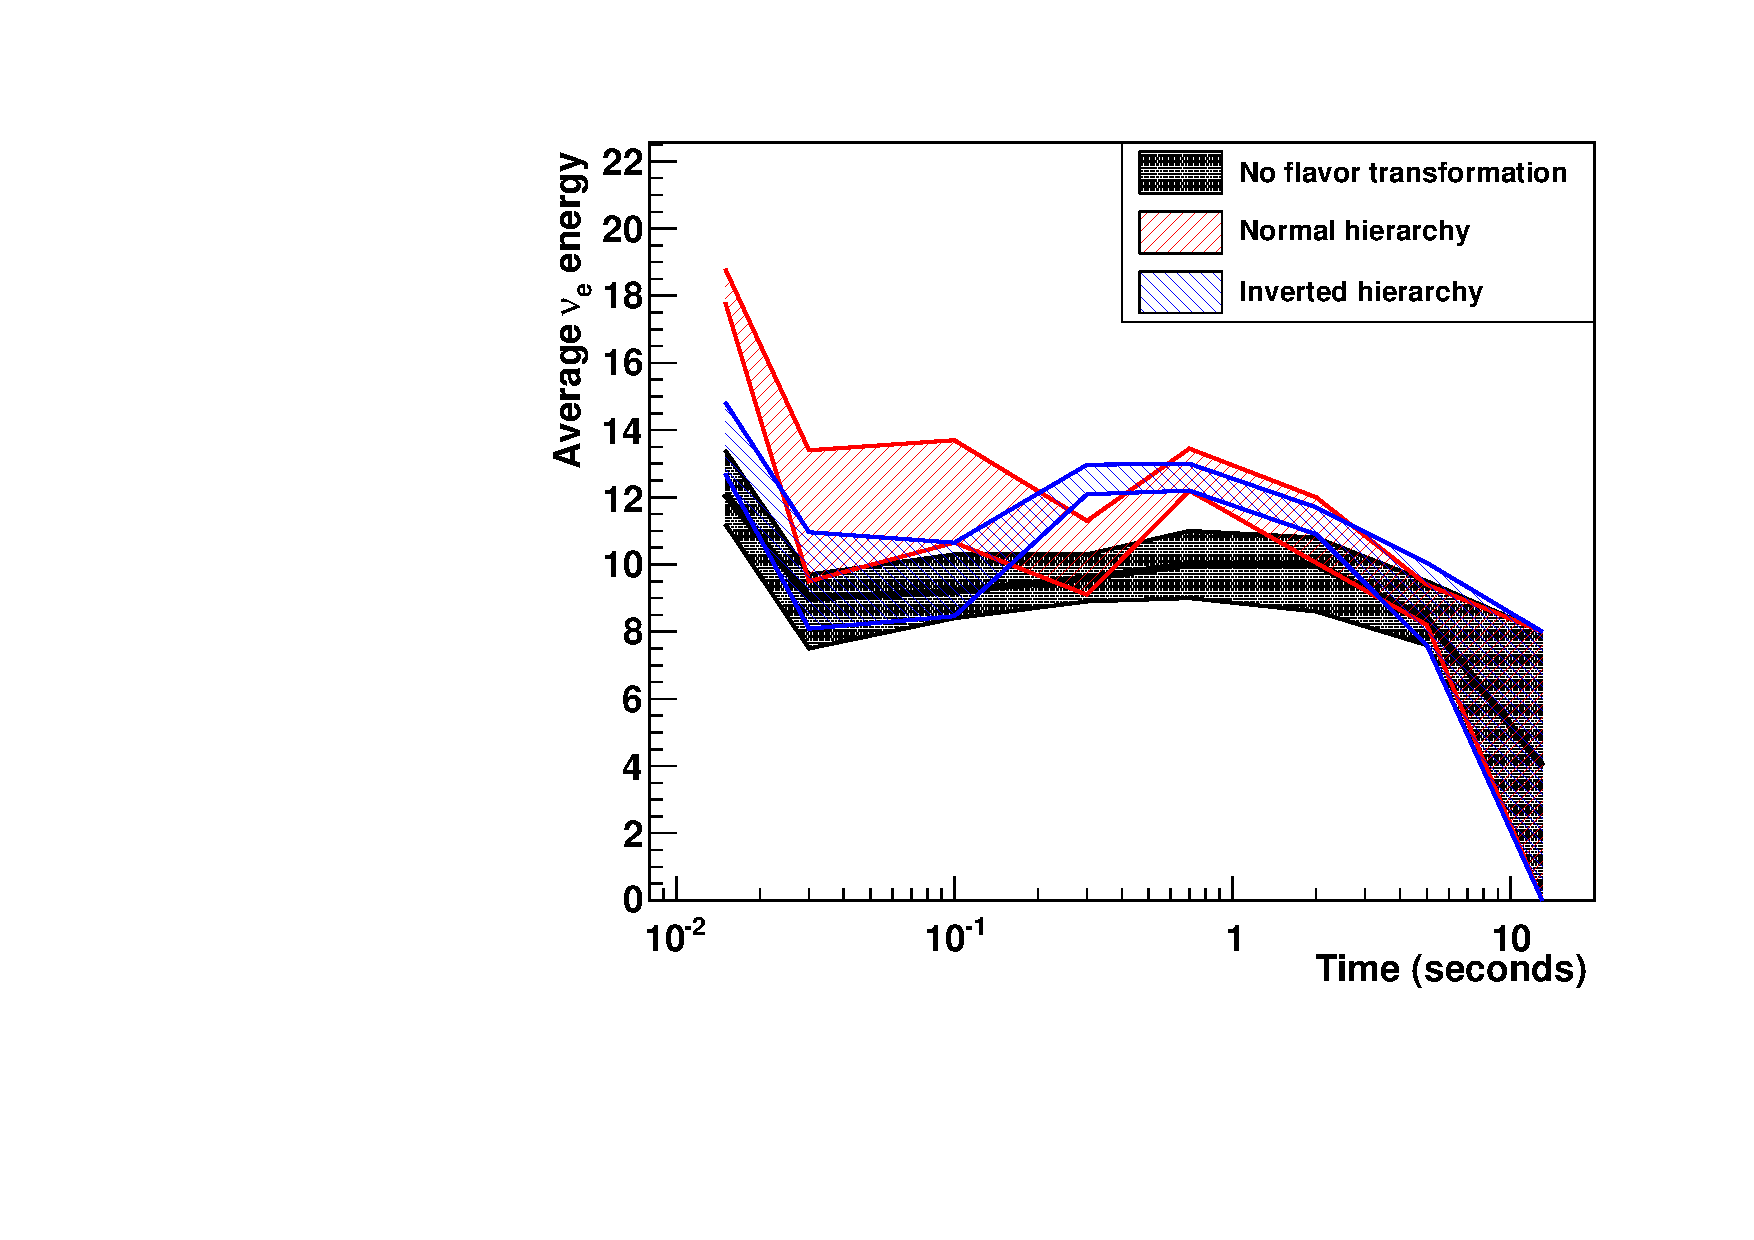
\includegraphics[width=0.9\textwidth]{timedep.pdf}
\end{cdrfigure}


The analysis of possible supernova events will make use of two types of information. First, the total energy of the emitted neutrinos will be compared with the expected release in the gravitational collapse.  Note that measurements of all flavors, including $\nu_e$, are needed for the best estimate of the energy release.
Second, the rate of cooling of the proto-neutron state should be measured and compared with what is expected from diffusion of the standard neutrinos. This requires comparing one-second-interval time-integrated spectra successively %at successive times 
as illustrated in Figure~\ref{fig:coolingcurves}. 

Because DUNE is mostly sensitive to $\nu_e$, in order to enable inference of the fluxes of $\mu$ and $\tau$ flavors complementary $\bar\nu_{e}$ measurements are needed from water Cherenkov and scintillator detectors, as is a careful analysis of the oscillation pattern (see below). Measuring the energy loss rate will require sufficient statistics at late times and, once again, an understanding of the oscillation dynamics; this is evident in Figure~\ref{fig:coolingcurves} where oscillated and unoscillated cases are shown.

%The flavor oscillation physics and its signatures are a major part of the physics program. Compared to the well-understood case of solar neutrinos, in a supernova, neutrino flavor transformations are much more involved. Not only neutrinos and antineutrinos of all flavors are emitted, not only are there two mass splittings -- ``solar'' and ``atmospheric'' -- to worry about, but the physics of the transformations is significantly richer. For example, several seconds after the onset of the explosion, the flavor conversion probability is affected by the expanding shock front and the turbulent region behind it. The conversion process in such a stochastic profile is qualitatively different from the adiabatic MSW effect in the smooth, fixed density profile of the Sun. 

The flavor oscillation physics and its signatures are a major part of the physics program. Compared to the well understood case of solar neutrinos, supernova neutrino flavor transformations are much more involved. Besides the facts that neutrinos and antineutrinos of all flavors are emitted and there are two mass splittings -- ``solar'' and ``atmospheric'' --  the physics of the transformations is significantly richer. For example, several seconds after the onset of the explosion, the flavor conversion probability is affected by the expanding shock front and the turbulent region behind it. The conversion process in such a stochastic profile is qualitatively different from the adiabatic MSW effect in the smooth, fixed-density profile of the Sun. 

Even more complexity is brought about by the coherent scattering of neutrinos off each other. This neutrino ``self-refraction'' 
 results in highly nontrivial flavor transformations close to the neutrinosphere, typically within a few hundred kilometers from the center, where the density of streaming neutrinos is very high. Since the evolving flavor composition of the neutrino flux feeds back into the oscillation Hamiltonian, the problem is \emph{nonlinear}. Furthermore, as the interactions couple neutrinos and antineutrinos of different flavors and energies, the oscillations are characterized by \emph{collective} modes.  %This leads to very rich physics that has been the subject of intense interest over the last decade. A voluminous literature exists exploring these collective phenomena, e.g.,~\cite{Duan:2005cp,Fogli:2007bk,Raffelt:2007cb,Raffelt:2007xt,EstebanPretel:2008ni, Duan:2009cd,Dasgupta:2009mg,Duan:2010bg,Duan:2010bf,Wu:2014kaa}.  This is an active theoretical field and the effects are not yet fully understood. 
This leads to very rich physics that has been the subject of intense theoretical interest over the last decade. A voluminous literature exists exploring these collective phenomena,
e.g.,~\cite{Duan:2005cp,Fogli:2007bk,Raffelt:2007cb,Raffelt:2007xt,EstebanPretel:2008ni,
Duan:2009cd,Dasgupta:2009mg,Duan:2010bg,Duan:2010bf,Wu:2014kaa} the effects of which are not yet fully understood. 
A supernova burst is the only opportunity to study neutrino-neutrino interactions experimentally.

\begin{cdrfigure}[Simulated cooling curves from the Garching light progenitor model]{shockandcollective}{Both panels show solid lines that represent the simulated unoscillated $\nu_e$ (green, cooler) and $\nu_x$ (blue, hotter) fluxes. The filled curve shows the observed flux after the collective oscillations in the absence of (left) and presence of (right) the shock front. (Flux is shown in arbitrary units)}
%A simulation of the effects of collective oscillations alone (left panel) and of collective oscillations plus the shock front (right panel). The solid lines represent unoscillated $\nu_e$ (green, cooler) and $\nu_x$ (blue, hotter) flux, and the filled curve shows the observed flux after the collective oscillations in both cases. (Flux is shown in arbitrary units)
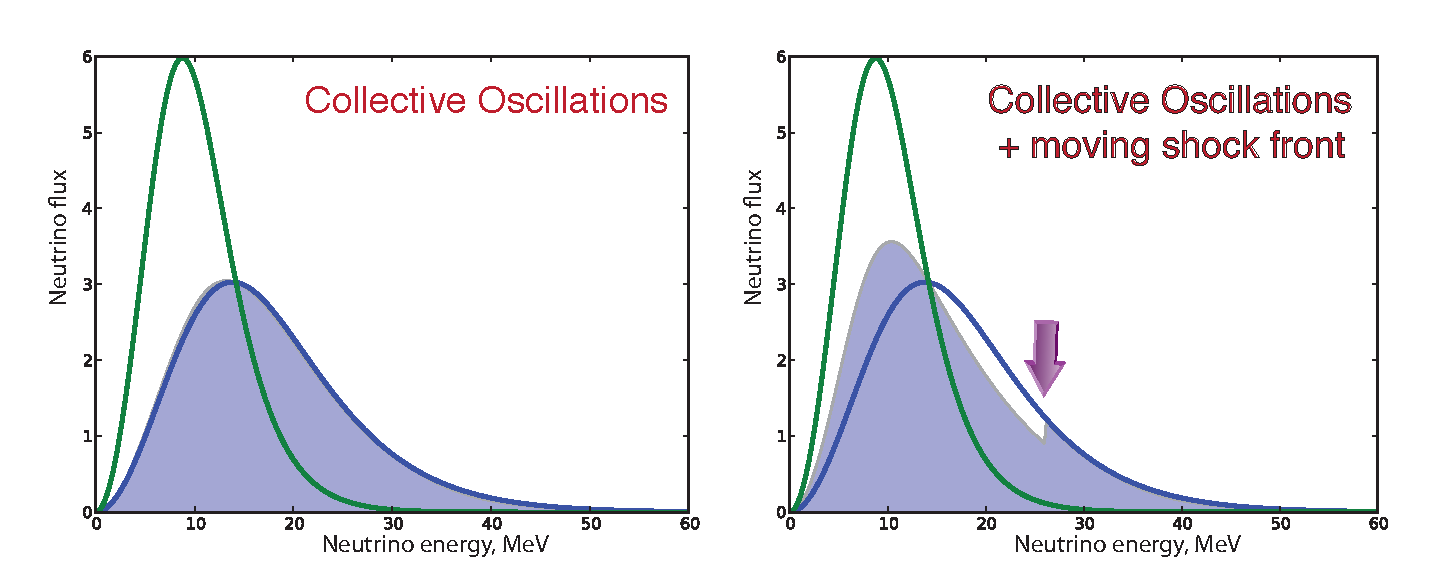
\includegraphics[width=0.9\textwidth]{shockandcollective.pdf}
\end{cdrfigure}

Matter effects in the Earth can also have a MH-dependent effect on the signal (e.g.,~\cite{Choubey:2010up}).

One may wonder whether all this complexity will impede the extraction of useful information from the future signal. In fact, the opposite is true: the new effects can \emph{imprint} information about the inner workings of the explosion on the signal. The oscillations can modulate the characteristics of the signal (both event rates and spectra as a function of time), as seen in Figure~\ref{fig:coolingcurves}. Moreover, the oscillations can imprint \emph{non-thermal} features on the energy spectra, potentially making it possible to disentangle the effects of flavor transformations and the physics of neutrino spectra formation. This in turn should help %us learn about 
illuminate the development of the explosion during the crucial first 10 seconds.   It is important to note that the features depend on the unknown mass hierarchy, and therefore may help reveal it. %tell us what the hierarchy is.

Figure~\ref{fig:shockandcollective} illustrates the effects of collective oscillations. %The role of the collective oscillations in this case is to 
These oscillations serve to permute almost completely the original $\nu_{e}$ and $\nu_{\mu,\tau}$ spectra, so that the flux of observed electron neutrinos is noticeably hotter than the original one. Moreover, the shock front modulates the MSW conversion probability and imprints a non-thermal \emph{step} in the spectrum.  Below this step, the swap between the original $\nu_{e}$ and $\nu_{\mu,\tau}$ spectra is only partial. As the shock expands, the feature moves to higher energies, creating a ``smoking-gun'' signature that exists only in the neutrino channel. 




% From Alan Kostelecky
%As another example of a probe of new physics with supernova neutrinos or antineutrinos,a class of tests of Lorentz and CPT violation involves comparing the propagation of neutrinos with other species or of neutrinos of the same flavor but different energies~\cite{Kostelecky:2003cr,Kostelecky:2003xn,Kostelecky:2011gq,Diaz:2009qk}. These amount to time-of-flight or dispersion studies.Time-of-flight and dispersion effects lack the interferometric resolving power available to neutrino oscillations, but they provide instead sensitivity to Lorentz- and CPT-violating effects that cannot be detected via oscillations. The corresponding SME coefficients controlling these effects are called oscillation-free coefficients~\cite{Kostelecky:2011gq}.Supernova neutrinos are of particular interest in this context because of the long baseline, which implies sensitivities many orders of magnitude better than available from time-of-flight measurements in beams. Observations of the supernova SN1987A yield constraints on the difference between the speed of light and the speed of neutrinos, which translates into constraints on isotropic and anisotropic coefficients in both the minimal and nonminimal sectors of the SME. Knowledge of the spread of arrival times constrains the maximum speed difference between SN1987A antineutrinos of different energies in the approximate range 10--40 MeV, which restricts the possible antineutrino dispersion and yields further constraints on SME coefficients~\cite{Kostelecky:2011gq}.Analyses of this type would be possible with DUNE if supernova neutrinos are observed. Key features to maximize sensitivity would include absolute timing information to compare with photon spectral observations and relative timing information for different components of the neutrino energy spectrum. Significant improvements over existing limits are possible.Figure 4 displays DUNE supernova sensitivities to coefficients for Lorentz and CPT violation that leave unaffected neutrino oscillations and so cannot be measured using atmospheric or long-baseline neutrinos. The figure assumes a supernova comparable to SN1987A (optimistically at a distance of 50 kpc). Studies of supernova neutrinos using DUNE can measure many coefficients (green) at levels improving over existing limits (grey).

As another example of a probe of new physics with supernova neutrinos or antineutrinos,
a class of tests of Lorentz and CPT violation involves comparing the propagation of neutrinos with other species or of neutrinos of the same flavor but different energies~\cite{Kostelecky:2003cr,Kostelecky:2003xn,Kostelecky:2011gq,Diaz:2009qk}. These amount to time-of-flight or dispersion studies.

Time-of-flight and dispersion effects lack the interferometric resolving power available to neutrino oscillations, but they provide sensitivity to Lorentz- and CPT-violating effects that cannot be detected via oscillations. The corresponding SME coefficients controlling these effects are called oscillation-free coefficients~\cite{Kostelecky:2011gq}.
Supernova neutrinos are of particular interest in this context because of the long baseline, which implies sensitivities many orders of magnitude greater than available from time-of-flight measurements in beams. Observations of the supernova SN1987A yield constraints on the difference between the speed of light and the speed of neutrinos, which translates into constraints on isotropic and anisotropic coefficients in both the minimal and nonminimal sectors of the SME. Knowledge of the spread of arrival times constrains the maximum speed difference between SN1987A antineutrinos of different energies in the approximate range 10--40 MeV, which restricts the possible antineutrino dispersion and yields further constraints on SME coefficients~\cite{Kostelecky:2011gq}.
\fixme{Milind dec2015: let's rewrite this later}

Analyses of this type would be possible with DUNE if supernova neutrinos are observed. Key features for maximizing sensitivity would include absolute timing information to compare with photon spectral observations and relative timing information for different components of the neutrino energy spectrum. Significant improvements over existing limits are possible.
Figure~\ref{fig:snliv} displays DUNE supernova sensitivities to coefficients for Lorentz and CPT violation that leave neutrino oscillations unaffected and so cannot be measured using atmospheric or long-baseline neutrinos. The figure assumes a supernova comparable to SN1987A (optimistically at a distance of 50~kpc). Studies of supernova neutrinos using DUNE can measure many coefficients (green) at levels that improve on existing limits (grey).


\begin{cdrfigure}[DUNE SN sensitivities to oscillation-free coefficients for Lorentz and CPT violation]{snliv}{DUNE supernova sensitivities to oscillation-free coefficients for Lorentz and CPT violation. Studies of DUNE supernova neutrinos can measure many coefficients (green) at levels improving over existing limits (grey). These Lorentz- and CPT-violating effects leave oscillations unchanged and so are unobservable in atmospheric or long-baseline measurements~\cite{kostelecky}.}
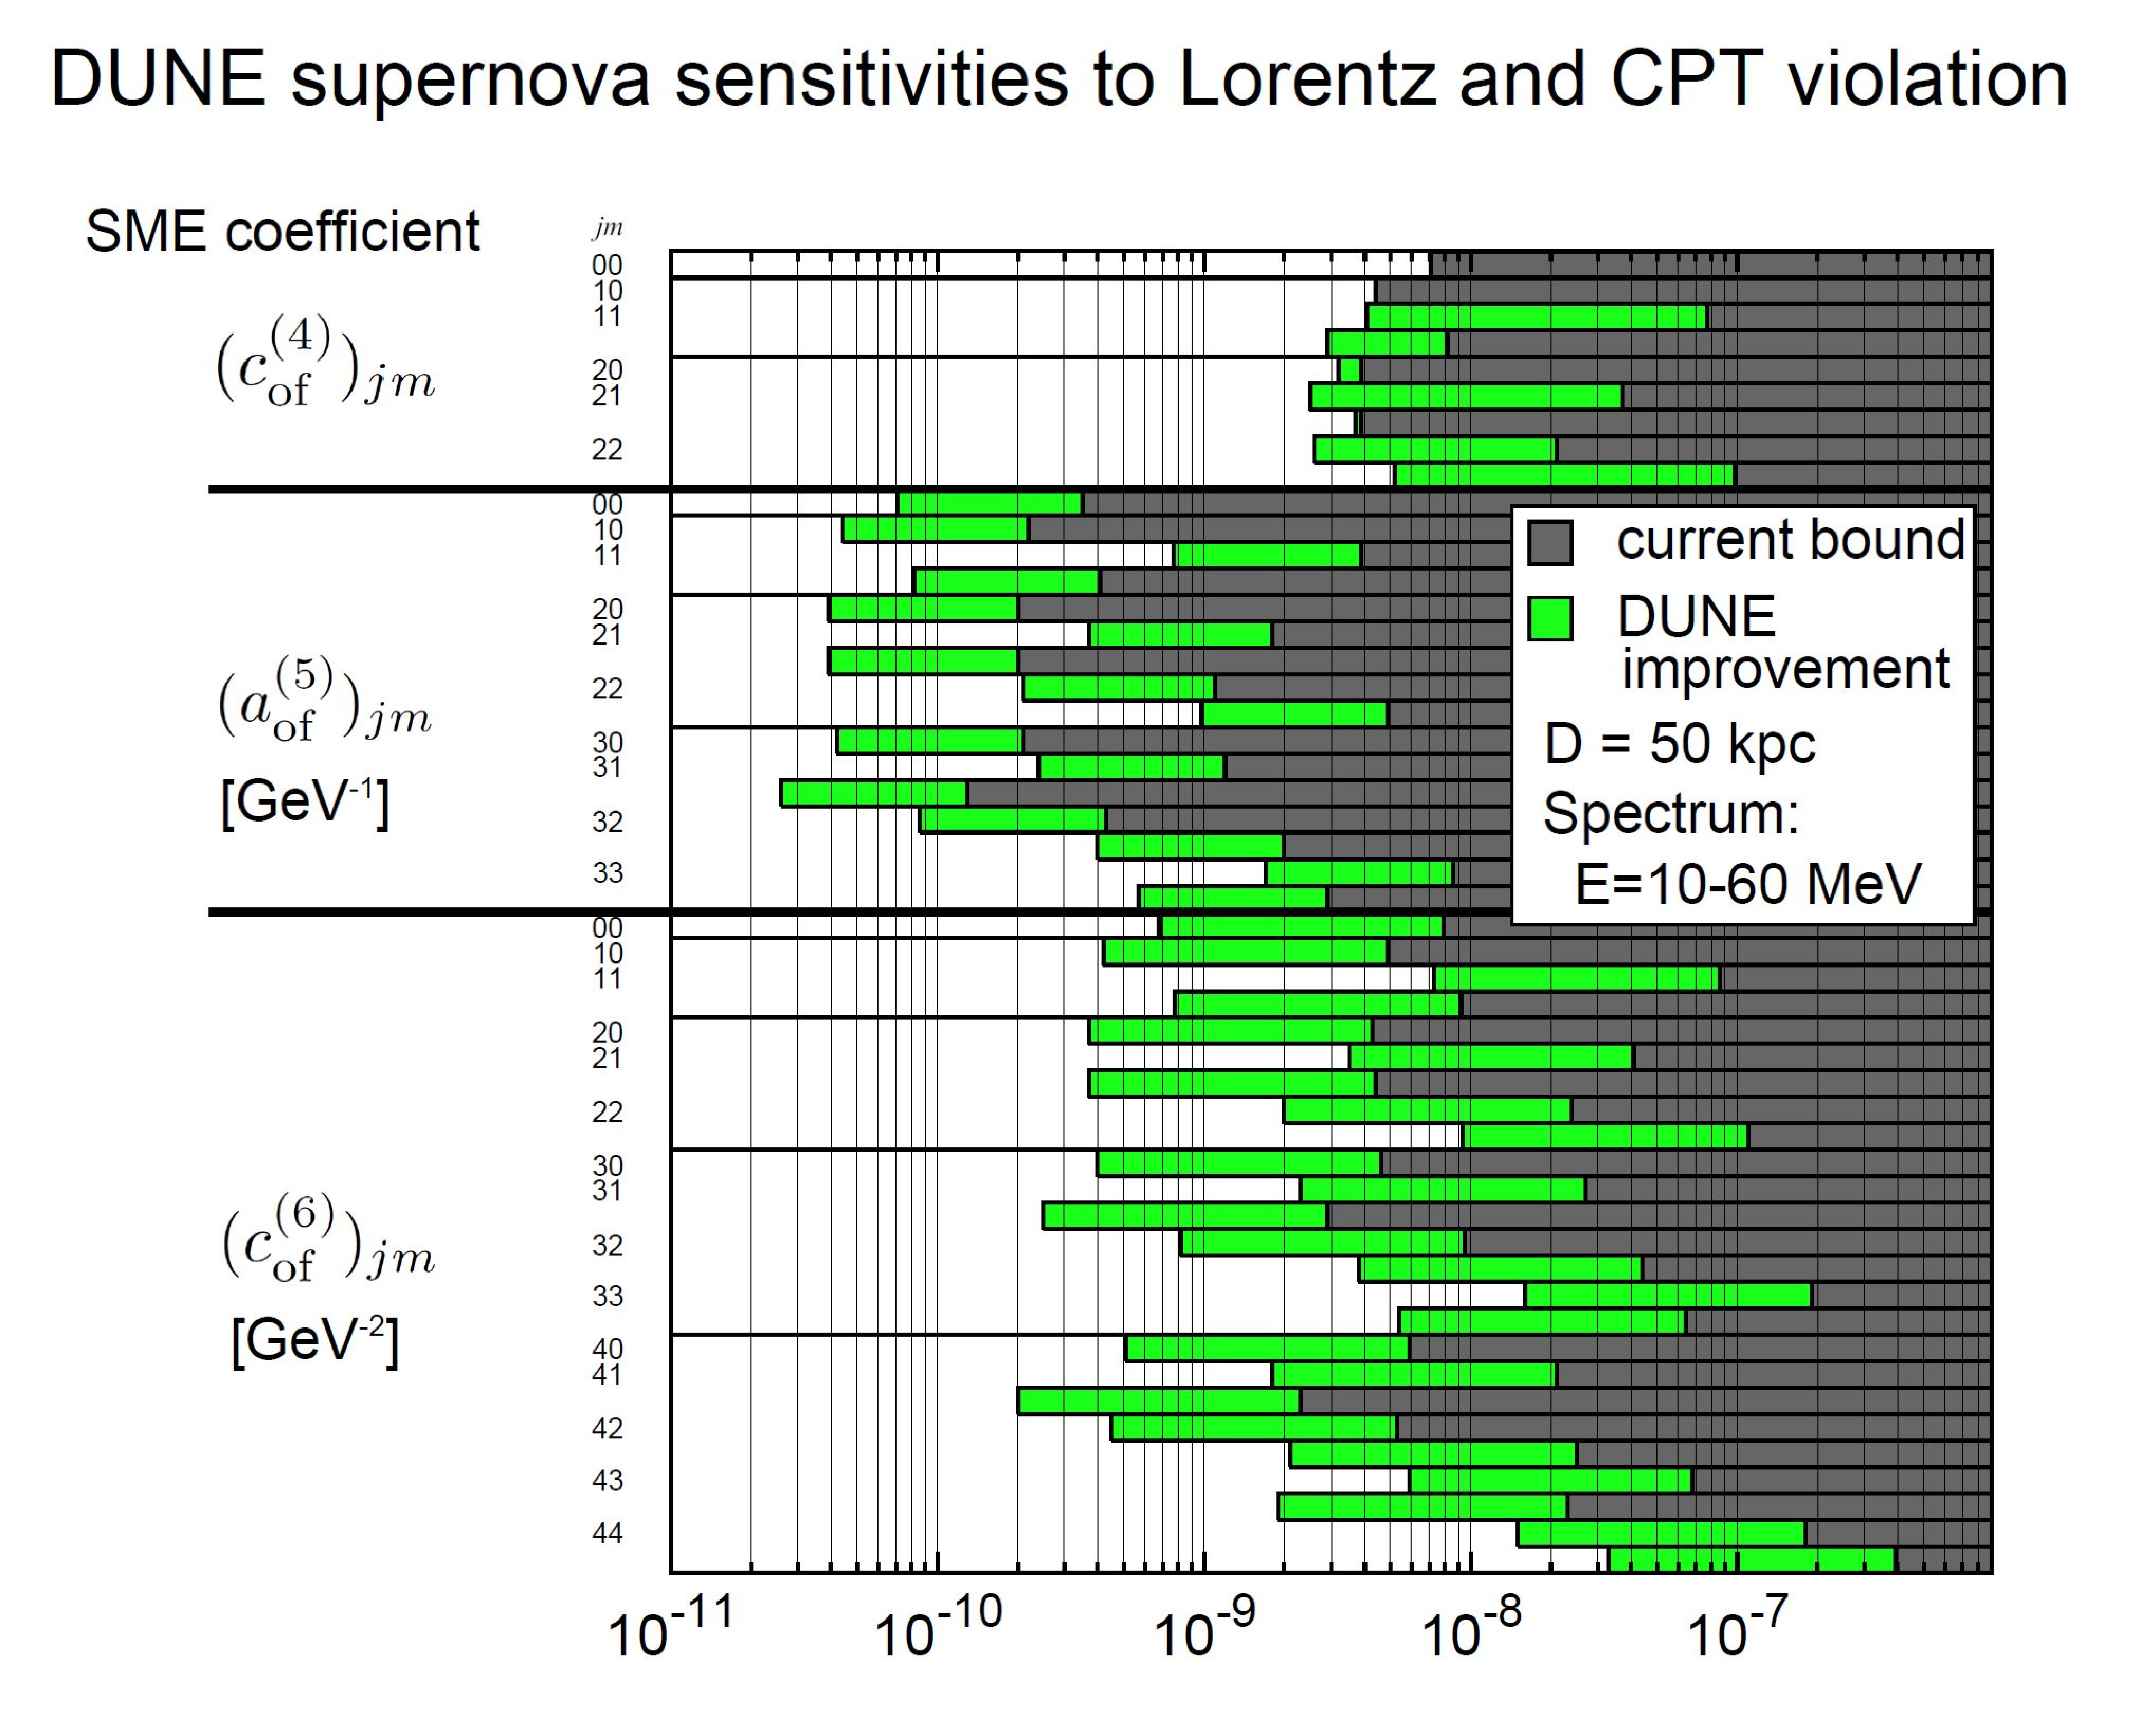
\includegraphics[width=0.9\textwidth]{DUNE-SME-SN.pdf}
\end{cdrfigure}

Finally, via detection of time-of-flight delayed $\nu_e$ from the  neutronization burst,  DUNE will be able to probe neutrino mass bounds of $\mathcal{O}(1)$~eV for a 10-kpc supernova~\cite{Rossi-Torres:2015rla} (although will likely not be competitive with near-future terrestrial kinematic limits). If eV-scale sterile neutrinos exist, they will likely have an impact on astrophysical and oscillation aspects of the signal (e.g.,~\cite{Keranen:2007ga,Tamborra:2011is,Esmaili:2014gya}), as well as time-of-flight observables. 


\section{Astrophysics}
\label{sec:physics-snblowe-astrophysics}


A number of astrophysical phenomena associated with supernovae are expected to be observable
in the supernova neutrino signal, providing a remarkable window into the event.  In particular, the supernova explosion mechanism, which in the current paradigm involves energy deposition via neutrinos, is still not well understood, and the neutrinos themselves will bring the insight needed to confirm or refute the paradigm.

There are many other examples of astrophysical observables.
\begin{itemize}
\item The short initial ``neutronization'' burst, primarily composed of $\nu_e$, %and called the or ``breakout'' burst, 
  represents only a small component of the total signal.  However,
  oscillation effects can manifest themselves in an observable manner
  in this burst, and flavor transformations can be modified by the
  ``halo'' of neutrinos generated in the supernova envelope by
  scattering~\cite{Cherry:2013mv}. 
  
\item The formation of a black hole would cause a sharp signal cutoff
  (e.g.,~\cite{Beacom:2000qy,Fischer:2008rh}).
\item Shock wave effects (e.g.,~\cite{Schirato:2002tg}) would cause a
  time-dependent change in flavor and spectral composition as the
  shock wave propagates.
\item The standing accretion shock instability
  (SASI)~\cite{Hanke:2011jf,Hanke:2013ena}, a ``sloshing'' mode
  predicted by three-dimensional neutrino-hydrodynamics simulations of
  supernova cores, would give an oscillatory flavor-dependent
  modulation of the flux.
\item Turbulence effects~\cite{Friedland:2006ta,Lund:2013uta} would
  also cause flavor-dependent spectral modification as a function of
  time.
\end{itemize}

Observation of a supernova neutrino burst in coincidence with gravitational waves (which would also be prompt, and could indeed provide a time reference for a time-of-flight analysis) would be especially interesting~\cite{Arnaud:2003zr,Ott:2012jq, Mueller:2012sv, Nishizawa:2014zna}.

The supernova neutrino burst is prompt with respect to the
electromagnetic signal and therefore can be exploited to provide an
early warning to astronomers~\cite{Antonioli:2004zb,Scholberg:2008fa}.  
Additionally, a liquid argon signal~\cite{Bueno:2003ei} is expected to
provide some pointing information, primarily from elastic scattering
on electrons.
We note that not every core collapse will produce an observable supernova, and observation of a neutrino burst in the absence of light would be very interesting. 

Even non-observation of a burst, or non-observation of
a $\nu_e$ component of a burst in the presence of supernovae (or other
astrophysical events) observed in electromagnetic or gravitational
wave channels, would still provide valuable information about the
nature of the sources.  Further, a long-timescale, sensitive search
yielding no bursts will also provide limits on the rate of
core-collapse supernovae.

We note that the better one can understand the astrophysical nature of core-collapse supernovae, the easier it will be to extract information about particle physics.  DUNE's capability to characterize the $\nu_e$ component of the signal is unique and critical.


\section{Additional Astrophysical Neutrinos}
\label{sec:physics-snblowe-other}

\subsection{Solar Neutrinos}

Intriguing questions in solar neutrino physics remain,
even after data
from the Super-K and SNO~\cite{Fukuda:2001nj,Ahmad:2001an}
experiments explained the long-standing mystery of missing solar
neutrinos~\cite{Cleveland:1998nv} as due to flavor
transformations. 
Some unknowns, such as the fraction of energy production via the CNO
cycle in the Sun, flux variation due to helio-seismological modes that
reach the solar core, or long-term stability of the solar core
temperature, are astrophysical in nature. Others directly impact
particle physics. Can the MSW model explain the amount of flavor
transformation as a function of energy, or are non-standard neutrino
interactions required?  Do solar neutrinos and reactor antineutrinos
oscillate with the same parameters? 

Detection of solar and other low-energy neutrinos is challenging in
a LArTPC because of relatively high intrinsic detection energy thresholds for
the charged-current interaction on argon ($>$\SI{5}{\MeV}). 
Compared with other technologies, a LArTPC offers a large
cross section and unique potential signatures from de-excitation
photons. Aggressive R\&D efforts in low-energy triggering and
control of background from radioactive elements may make detection
of solar neutrinos in DUNE possible.

Signatures of solar neutrinos in DUNE
are elastic scattering on electrons as well as CC absorption of $\nu_e$ on $^{40}$Ar (equation~\ref{eq:nueabs}), which has a 4.5-MeV energy threshold and a large cross section compared to elastic scattering on electrons.  Furthermore, the CC absorption differential cross section (the interaction products track neutrino energy closely) potentially enables precise solar-neutrino spectral measurements.
The solar neutrino event rate in a
\ktadj{40} LArTPC, assuming a roughly \MeVadj{4.5} neutrino energy
threshold and 31\% $\nu_e$ survival, is 122 per day.


The solar neutrino physics potential of a large LArTPC depends
on the ability to pick up a low-energy electron, light collection of the photon-triggering system,
and, critically, on background suppression. 
The decay of the naturally occurring $^{39}$Ar
produces $\beta$'s with a \keVadj{567} endpoint and an expected rate
of \SI{10}{\MHz} per \SI{10}{\kt} of liquid argon. This limits the
fundamental reach of DUNE to neutrino interactions with visible
energies above \SI{1}{\MeV}. 
Cosmic-muon and fast-neutrino  interactions with the $^{40}$Ar nucleus (which are rather complex
compared to interactions on $^{16}$O or $^{12}$C) are likely to generate many long-lived spallation products which could limit the
detection threshold for low-energy neutrinos.
$^{40}$Cl, a beta emitter with an
endpoint of \SI{7.48}{\MeV}, is a dominant source of background at
energies above \SI{5}{\MeV}, and is expected to be produced with a rate on the order of 10 per kiloton of LAr per day at 4850 ft.



The ICARUS collaboration has reported a \MeVadj{10}
threshold~\cite{Guglielmi:2012}. Assuming the detector itself
has low enough radioactivity levels, this threshold level would enable
a large enough detector to measure the electron flavor component of
the solar $^8$B neutrino flux with high statistical accuracy. It could 
thereby further test the MSW flavor transformation curve with higher statistical precision and
potentially better energy resolution. 
In addition to these solar
matter effects, solar 
neutrinos also probe terrestrial matter effects
with the variation of the $\nu_e$ flavor observed with solar zenith
angle while the Sun is below the horizon --- the day/night effect (reported recently in ~\cite{Renshaw:2013dzu}). 
%The comparison of neutrino disappearance to antineutrino disappearance tests CPT invariance. 
The comparison of solar and reactor disappearance tests CPT invariance as well as other new physics.

\subsection{Diffuse Supernova Background Neutrinos}

Galactic supernovae are relatively rare, occurring somewhere between
once and four times a century. In the Universe
at large, however, thousands of neutrino-producing explosions occur
every hour.  The resulting neutrinos --- in fact most of the neutrinos
emitted by all the supernovae since the onset of stellar formation ---
suffuse the Universe.  Known as the \emph{diffuse supernova neutrino background
  (DSNB)}, their energies are in the few-to-\MeVadj{30} range.  The DSNB
has not yet been observed, but an observation would greatly enhance
our understanding of supernova-neutrino emission and the overall
core-collapse rate~\cite{Beacom:2010kk}.


A liquid argon detector such as DUNE's far detector is sensitive to
the $\nu_e$ component of the diffuse relic supernova neutrino flux,
whereas water Cherenkov and scintillator detectors are sensitive to
the antineutrino component.  However, backgrounds in liquid argon are as
yet unknown, and a huge exposure ($>$\SI{500}{\ktyr}s)
would likely be required for observation.  
With tight control of
backgrounds, 
DUNE --- in the long term --- could play a unique and
 complementary role in the physics of relic neutrinos.


Background is a serious issue for DSNB detection.
The solar {\em hep} neutrinos, which have an                
endpoint at \SI{18.8}{\MeV}, will determine the lower bound of the DSNB
search window ($\sim$ \SI{16}{\MeV}).  The upper bound is determined
by the atmospheric ${\nu}_{e}$ flux and
is around \SI{40}{MeV}.
Although the LArTPC provides a unique sensitivity to the
electron-neutrino component of the DSNB flux, early studies indicate
that due to this lower bound of $\sim$ \SI{16}{\MeV}, DUNE would need a huge
mass of liquid argon --- of order \SI{100}{\kt} --- to get more than 4$\sigma$
evidence for the diffuse supernova flux in five
years~\cite{Cocco:2004ac}.
%
The expected number of relic
supernova neutrinos, $N_{\rm DSNB}$, that could be observed in a
\SIadj{40}{\kt} LArTPC detector in ten years~\cite{Cocco:2004ac}
assuming normal hierarchy is:
\begin{equation}
N_{\rm DSNB} = 46 \pm 10  \ \ \ 16 \, {\rm MeV} \leq E_e \leq 40 \, {\rm MeV}
\label{eqn:srnrate}
\end{equation}
where $E_e$ is the energy of the electron from the CC interaction as
shown in Equation~\ref{eq:nueabs}. 

 The main challenge for detection of such
a low rate of relic neutrinos in a LArTPC is understanding how much of
the large spallation background from cosmic-ray interactions with the
heavy argon nucleus 
leaks into the search window.   Some studies have been done~\cite{Barker:2012nb} but more work is needed.

\subsection{Other Low-Energy Neutrino Sources}

We note some other potential sources of signals in the tens-of-MeV range that may be observable in DUNE.  These include neutrinos from accretion disks~\cite{Caballero:2011dw} and black-hole/neutron star mergers~\cite{Caballero:2009ww}.  These will create spectra not unlike those from core-collapse events, and with potentially large fluxes.  However they are expected to be considerably rarer than core-collapse supernovae within an observable distance range.  There may also be signatures of dark-matter WIMP annihilations in the low-energy signal range~\cite{Rott:2012qb, Bernal:2012qh}.



\section{Detector Requirements}
\label{sec:physics-snblowe-detector-requirements}

For supernova burst physics, the detector must be able to detect and reconstruct %as well as possible \fixme{sounds like a weasely kind of `must' (Maury says to leave it)} 
events in the range 5--100~MeV.  As for proton decay and atmospheric neutrinos, no beam trigger will be available; therefore there must be special triggering and DAQ requirements that take into account the short, intense nature of the burst, and the need for prompt propagation of information in a worldwide context.
The DUNE Far Detector
Requirements~\cite{lbnfdune-cdr-req} specific to supernova burst neutrinos are as follows:

\begin{itemize}

\item Far Detector Depth: The signal to background ratio shall be sufficiently large to identify the  burst ($<$100 seconds)  from a core-collapse supernova within 20~kpc (within the Milky Way). This will require a detector located at sufficient depth for cosmic-ray-related background, including spallation-induced events, to be sufficiently low.  Furthermore, backgrounds from radioactivity or other sources must also be sufficiently low.  Preliminary studies~\cite{gehman} indicate that backgrounds at 4850 ft (including both cosmogenics and intrinsic radioactivity) will be sufficiently low, although more work is needed. \fixme{It says `sufficiently low' three times without saying what constitutes `sufficiently low' Maury says leave it for now}

\item Far Detector Triggering and DAQ:  The far detector shall be capable of collecting information for a supernova burst within the Milky Way.  Events are expected within a time window of approximately 10 seconds, but possibly over an interval as long as several tens of seconds; a large fraction of the events are expected within approximately the first second of the burst.
The data acquisition buffers shall be sufficiently large and the data acquisition system sufficiently robust to allow full capture of neutrino event information for a supernova as close as 0.1 kpc.
At 10~kpc, one expects thousands of events within approximately 10 seconds, but a supernova at a distance of less than 1~kpc would result in $10^5-10^7$  events over 10 seconds.    

The far detector shall have high uptime ($>$90\%) with little event-by-event deadtime to allow the capture of low-probability astrophysical events that could occur at any time with no external trigger. 
Supernova events are expected to occur a few times per century within the Milky Way galaxy. For any 10-year period, the probability of a supernova could be 20 to 30\%.  Capturing such an event at the same time as many of the other detectors around the Earth is very important.  

The DUNE detector systems shall be configured to provide  information to other observatories on possible astrophysical events (such as a galactic supernova) in a short enough time to allow global coordination.   
To obtain maximum scientific value out of a singular astronomical event, it is very important to inform all other observatories (including optical ones) immediately, so that they can begin observation of the evolution of the event. 

\item Far Detector Event Reconstruction:   
The far detector shall be capable of collecting low energy ($<$\SI{100}{\MeV})  charged-current electron neutrino interactions on $^{40}$Ar nuclei that arrive in a short period of time. The final-state electron (or positron) shall be detected and its energy measured.   An energy threshold of 5 MeV or better is highly desirable; most supernova burst events are expected to have energy depositions in the range 5--50~MeV.
Energy and event time resolution must be sufficient to resolve interesting physics features of the burst.  Preliminary studies suggest that resolution measured by Icarus for low-energy events~\cite{Amoruso:2003sw} should be adequate, and that approximately millisecond event time resolution should be sufficient to resolve features such as the neutronization burst and the preceding short notch due to neutrino trapping in the $\nu_e$ spectrum (see the luminosity curve of Figure~\ref{fig:garching}), given adequate statistics.   

Detection of gamma ray photons from the final-state excited nucleus could lead to additional electronics requirements.  

\end{itemize}



The other low-energy physics described in Section~\ref{sec:physics-snblowe-other} typically requires event reconstruction capabilities similar to supernova-burst physics; however, background requirements are much more stringent for these (especially for DSNB).  Realistic background conditions in the few-tens-of-MeV range are not currently  very well understood.  
These physics topics do not drive detector requirements, although it may still be possible for DUNE to address them if backgrounds can be kept sufficiently well under control.
